\section{Índices de governo eletrônico}

Existem 4 tipos de índices de governo eletrônico, segundo \cite{martinez2022egovernment}: EDGI da ONU, GTMI do Banco Mundial, DESI da Comissão Europeia da União Europeia e DGI da OECD.

A DESI não será usado porque o índice, administrado pela Comissão Europeia da UE, foca no análise individual de cada estado-membro da UE para que eles possam identificar áreas que precisam de ações prioritárias e capítulos temáticos que providenciam analises a nível supranacional em áreas de áreas chave de política digital.

\subsection{EGDI}

% DEFINIR O QUE EGDI

\subsubsection{Coeficiente de correlação de Pearson: EGDI, índice de democracia eleitoral e PIB \textit{per capital}}

Ao analisar os dados do \href{https://publicadministration.un.org/egovkb/en-us/About/Overview/-E-Government-Development-Index}{EGDI}, foi notado que tanto democracias consolidade, quanto autocracias históricas tem um EGDI alto. 

\begin{figure}[H]
    \centering
    \caption{Coeficiente de correlação de Pearson: índice de democracia e o EGDI da Rússia e Brasil}
    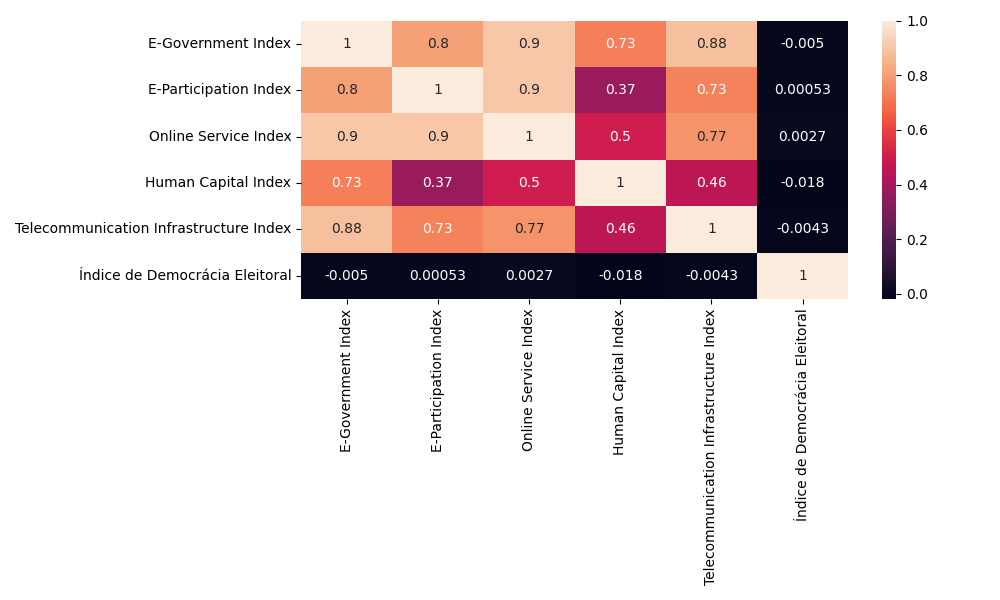
\includegraphics[width=1\linewidth]{figuras/egdi/correlacao3.png}
    \label{fig:correlacao3}
    \footnotesize{Fonte: baseado em \cite{ONU_edgi_mapa} e \cite{electoral_democracy_index}.}
\end{figure}

O coeficiente de correlação de Pearson entre -0.8 e -0.89 entre EGDI do Brasil e o IDE do Brasil e EGDI da Rússia e o IDE da Rússia. Como essa relação não respondeu o questionamento do parágrafo inicial. Buscou-se outro critério a ser comparado com o EGDI: o PIB \textit{per capita} do Brasil e Rusia. Para tanto, descrobiu-se o coeficiente de correlação de Pearson, cujo resultado está presente na figura \ref{fig:correlacao4}.

\begin{figure}[H]
    \centering
    \caption{Coeficiente de correlação de Pearson: índice de democracia e o PIB \textit{per capita} dos 193 países}
    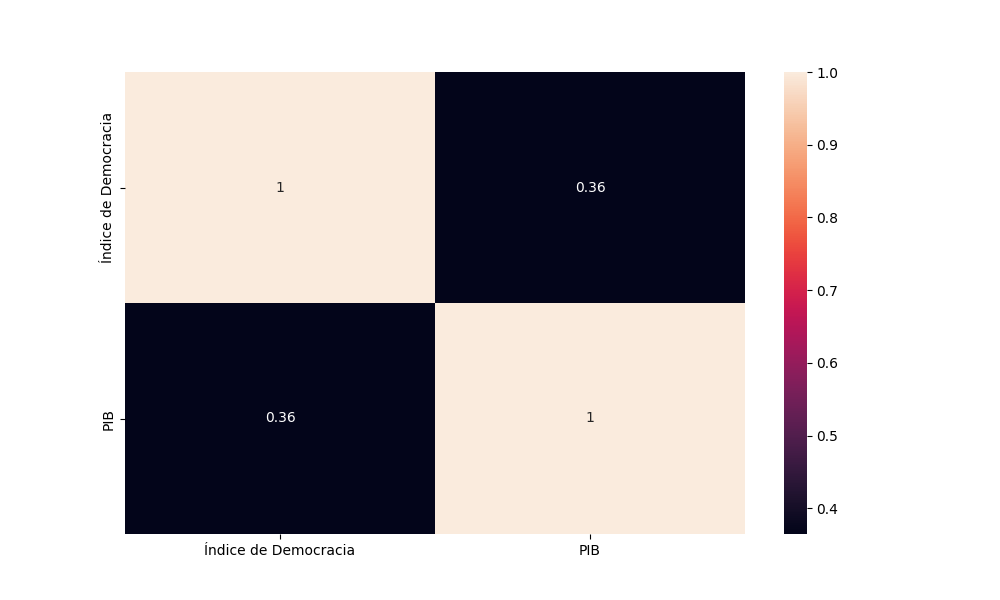
\includegraphics[width=1\linewidth]{figuras/egdi/correlacao4.png}
    \label{fig:correlacao4}
    \footnotesize{Fonte: baseado em \cite{ONU_edgi_mapa} e \cite{electoral_democracy_index}.}
\end{figure}

O coeficiente


%WB_pib_per_capita_paises e ONU_edgi_mapa